\section{Cómputo Ubicuo}

Es la integración de la informática en el entorno de la persona, de forma que los ordenadores no se perciban como objetos extraños.

Utilización de muchos dispositivos de computación que están presentes en los entornos físicos: casa, oficina y otros.

\begin{figure}[h!]
	\centering
		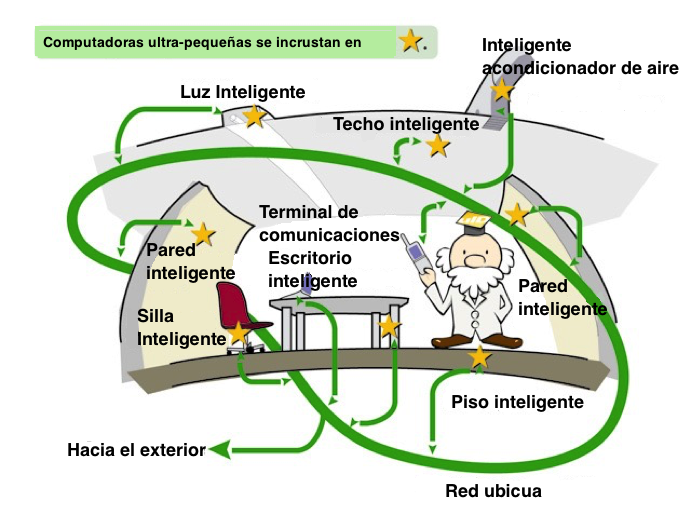
\includegraphics[width=0.8\textwidth]{Figuras/ubicuo.png}
		\rule{35em}{0.5pt}
	\caption[Integración de dispositivos inteligentes en el ambiente]{Integración de dispositivos inteligentes en el ambiente \cite{ubicuo}}
	\label{fig:ubicuo}
\end{figure}
